\documentclass[12pt,a4paper]{report}
\usepackage[a4paper,vmargin={1in,1in},hmargin={1.25in,1in}]{geometry}	% Setup of page size,margins
\usepackage{graphics}
\usepackage[font=small,labelfont=bf]{caption}
\usepackage{epsfig}
\usepackage{tabularx}
%\usepackage{algpseudocode}
%\usepackage{algorithm}
\usepackage{subfigure}  
\usepackage[titletoc]{appendix}
\renewcommand{\appendixname}{Annexure}
\usepackage{multirow}
\usepackage{fancyhdr}		% For special customization of headers and footers
\usepackage{fancybox}		% For formatting of cover page5
\usepackage{amsmath}    	% For  mathematical formulae
\usepackage{amsfonts}
\usepackage{amssymb}
\usepackage{textcomp}
\usepackage{setspace}		% For adjusting line spacing 
\usepackage{pdfpages}
\usepackage[square, comma, sort&compress,numbers]{natbib} % For customizing citations
%\usepackage[pdftex]{hyperref}	% For having working URLs for references 
\usepackage[colorlinks=true,linkcolor=blue,urlcolor=blue]{hyperref}
\usepackage[UKenglish]{isodate}
\usepackage[intoc]{nomencl}
\usepackage{multirow} 		  	% for row spannig in table environment
\usepackage{xcolor}
\definecolor{light-gray}{gray}{0.95}
\usepackage{footnote} 			% this package conflicts with xcolor.  So keep its order as is
\makenomenclature
\onehalfspacing
\author{}
 \title{TECHCARE}
\begin{document}
\pagenumbering{roman}
\pagestyle{empty}
%------------------------------------------------------------------------------
%   Cover Page starts here
%------------------------------------------------------------------------------
\newpage
\pagestyle{empty}
\pagenumbering{gobble}
%\thisfancypage{cmds1}{cmds2}
\thisfancyput(-0.0 in, -10.0 in) {\setlength{\unitlength}{1 in}\framebox(6.7,10.2)}

\begin{center}
	\vspace*{0.2 in}
	\textbf{\large{SAVITRIBAI PHULE PUNE UNIVERSITY}}\\
  \vspace*{0.25 in}
\textbf{A PROJECT REPORT ON}
\vspace{0.05 in}
  \end{center}
\vspace{0.05 in}
	\begin{center}
		\textbf{\large{TECHCARE}} \\
	\end{center}
	
	\vspace{0.1 in}
	\begin{center}
	SUBMITTED TOWARDS THE PARTIAL FULFILMENT OF THE REQUIREMENTS OF
\end{center}
	\vspace{0.1 in}
	\begin{center}
			\textbf{BACHELOR OF ENGINEERING(Computer Engineering)}
     	\end{center}
     \vspace{0.3 in}
		\begin{center}
	    BY
	\end{center}
	
	
	\begin{flushleft}
		\begin{flushleft}
\hspace{1.7in}\textbf{Adesh Tajane}
\hspace{0.38in}\textbf{  403080}\\
\hspace{1.7in}\textbf{Ronish Zadode}    
 \hspace{0.3in}\textbf{  403086}\\
\hspace{1.7in}\textbf{Ashutosh Kedar}\hspace{0.3in}\textbf{402065}\\
\hspace{1.7in}\textbf{Prabhat Pandey}\hspace{0.3in}\textbf{403049}\\
\end{flushleft}
	\end{flushleft}
\vspace{0.05 in}		
	\begin{center}
	  \textbf{UNDER THE GUIDANCE OF}\\
	  \vspace{0.075 in}
	 \textbf{ Prof. Shilpa Sonawani}(Internal Guide)\\
	  
	\end{center}
		%\vspace{0.2 in}
		
		\vspace{0.3 in}
\begin{center}

\includegraphics[width=3cm]{mitlogo}
\end{center}

		\begin{center}
	  \textbf{Department Of Computer Engineering}\\
\bf{MAEER’s MAHARASHTRA INSTITUTE OF TECHNOLOGY} \\
\textbf{Kothrud, Pune 411 038}\\
\textbf{2015-2016}
	\end{center}
%------------------------------------------------------------------------------
%  Cover ends here
%------------------------------------------------------------------------------

%------------------------------------------------------------------------------
%  Certificate starts here
%------------------------------------------------------------------------------
\newpage
\pagestyle{empty}
 %\thispagestyle{empty}
	\pagenumbering{gobble}
	\thisfancyput(-0.0 in, -10.0 in) {\setlength{\unitlength}{1 in}\framebox(6.7,10.2)}
\begin{center}
\begin{figure}[h]
\centering

\includegraphics[width=1.5 cm]{mitlogo}
\end{figure}
 MAHARASHTRA ACADEMY OF ENGINEERING AND EDUCATIONAL RESEARCH\textquoteright S\\ \bf \vspace {0.001 in}MAHARASHTRA INSTITUTE OF TECHNOLOGY\\ PUNE\\\vspace {0.001 in} DEPARTMENT OF COMPUTER ENGINEERING\\
\vspace {0.0001 in}
\end{center}
\vspace{0.0005 in}
\begin{center}
\textbf{\underline{C E R T I F I C A T E}}\\
\vspace{0.0005 in}
\end{center}
		\noindent
  				\setlength{\baselineskip}{1.45\baselineskip}
	\begin{center}
This is to certify that \\
\textbf{\large TECHCARE}\\
Submitted by\\
	\begin{flushleft}
		\begin{flushleft}
\hspace{1.7in}\textbf{Adesh Tajane}
\hspace{0.38in}\textbf{  403080}\\
\hspace{1.7in}\textbf{Ronish Zadode}    
 \hspace{0.3in}\textbf{  403086}\\
\hspace{1.7in}\textbf{Ashutosh Kedar}\hspace{0.3in}\textbf{402065}\\
\hspace{1.7in}\textbf{Prabhat Pandey}\hspace{0.3in}\textbf{403049}\\
\end{flushleft}
	\end{flushleft}
	
	is a bonafide work carried out by Students under the supervision of Prof. Shilpa Sonawani and it is submitted towards the partial fulfilment of the requirement of Bachelor of Engineering (Computer Engineering).
	\vspace{0.3 in}
		\begin{center}
	Prof. Shilpa Sonawani \hspace{0.95 in} \hspace{0.95 in} \hspace{0.95 in}Dr. V. Y. Kulkarni\\
	Internal Guide \hspace{0.9 in} \hspace{0.9 in} \hspace{0.9 in} \hspace{0.9 in} H.O.D.\\
	Dept. of Computer Engg. \hspace{0.7 in} \hspace{0.7 in} \hspace{0.7 in} Dept. of Computer Engg.\\

		Dr. L. K. Kshirsagar\\
		Principal\\
		Maharashtra Institute of Technology
	
	\vspace{0.3 in}
	
	Signature of Internal Examiner \hspace{0.7 in} \hspace{0.7 in} Signature of External Examiner
\end{center}

\pagenumbering{roman}
\begin{center}
	\textbf{PROJECT APPROVAL SHEET}\\
	\vspace{0.2 in}
	A Project title\\
	\vspace{0.1 in}
	\textbf{TECHCARE}\\
	\vspace{0.15 in}
	Is successfully completed by\\
	\begin{flushleft}
		\begin{flushleft}
\hspace{1.7in}\textbf{Adesh Tajane}
\hspace{0.38in}\textbf{  403080}\\
\hspace{1.7in}\textbf{Ronish Zadode}    
 \hspace{0.3in}\textbf{  403086}\\
\hspace{1.7in}\textbf{Ashutosh Kedar}\hspace{0.3in}\textbf{402065}\\
\hspace{1.7in}\textbf{Prabhat Pandey}\hspace{0.3in}\textbf{403049}\\
\end{flushleft}
	\end{flushleft}
	at\\
	\vspace{0.1 in}
\textbf{DEPARTMENT OF COMPUTER ENGINEERING}\\
	\vspace{0.1 in}
	\textbf{MAHARASHTRA INSTITUTE OF TECHNOLOGY}\\
	\vspace{0.1 in}
	\textbf{SAVITRIBAI PHULE PUNE UNIVERSITY,PUNE}\\
	\vspace*{0.1 in}
	\textbf{ACADEMIC YEAR 2017-2018}\\
	\vspace{0.9 in}
	Prof. Shilpa Sonawani \hspace{0.9 in}\hspace{0.9 in} \hspace{0.9 in}Dr. V. Y. Kulkarni\\
	Internal Guide \hspace{0.6 in}\hspace{0.6 in}\hspace{0.6 in} \hspace{0.6 in} \hspace{0.6 in}\hspace{0.6 in} H.O.D.\\
	Dept. of Computer Engg. \hspace{0.7 in} \hspace{0.7 in} \hspace{0.6 in} Dept. of Computer Engg.\\
\end{center}
\singlespace

	\end{center}

%------------------------------------------------------------------------------
%  Certificate ends here
%------------------------------------------------------------------------------
%------------------------------------------------------------------------------
%  Abstract starts here
%------------------------------------------------------------------------------
%\newpage
%\addcontentsline{toc}{section}{ABSTRACT}

\begin{abstract}
	
	\begin{normalsize}
		
		\hspace{6mm} The project is an application of data mining and machine learning techniques to the time series data of the disease development based on the temperature changes associated. The project also includes high end application of latest methodologies of prediction. It is a real time prediction model. It includes application on most widely used android platform with three tier application.
		
		\textbf{Keywords:}\\ 
		Data Mining, Risk Prediction, Machine Learning.
		
	\end{normalsize}
\end{abstract}
%------------------------------------------------------------------------------
%  Abstract ends here
%------------------------------------------------------------------------------
\newpage
%\addcontentsline{toc}{section}{ACKNOWLEDGMENT}
\pagestyle{plain}           %For displaying roman page nos
\begin{center}
\bf ACKNOWLEDGEMENT
\end{center}
\hspace*{0.6cm}It gives us great pleasure in presenting the preliminary project report on `TECHCARE'.\\

We would like to take this opportunity to thank our internal guide Prof. Shilpa Sonawani
for giving us all the help and guidance we needed. We are really grateful for
her kind support. Her valuable suggestions were very helpful.\\

We are also grateful to Dr. V. Y. Kulkarni, Head of Computer Engineering Department, Maharashtra Institute of Technology,Pune for her indispensable support, suggestions.\\




\begin{flushleft}
\hspace{3.7in}Adesh Tajane\\
\hspace{3.7in}Ronish Zadode\\
\hspace{3.7in}Prabhat Pandey\\
\hspace{3.7in}Ashutosh Kedar\\
\hspace{3.7in}(B.E. Computer Engineering)\\
\end{flushleft}

%------------------------------------------------------------------------------
%  Acknowledgement ends here


%------------------------------------------------------------------------------
%  TOC starts here
%------------------------------------------------------------------------------
\newpage

\tableofcontents
%------------------------------------------------------------------------------
%  List of Figures,tables starts here
%------------------------------------------------------------------------------

\newpage
{\setlength{\baselineskip}{1.5\baselineskip}
\listoffigures
%\addcontentsline{toc}{section}{List of Figures}
}
\newpage
{\setlength{\baselineskip}{1.5\baselineskip}
\listoftables
%\addcontentsline{toc}{section}{List of Tables}
}


%------------------------------------------------------------------------------


%\begin{center}
\chapter{\bf{SYNOPSIS}}
%\end{center}
\pagenumbering{arabic}     %For displaying arabic(1,2,3 ..) page nos
\pagestyle{fancy}
\fancyhead[RO]{\textit{\begin{small}TechCare\end{small}}}
\fancyhead[LO]{\textit{\begin{small}PROJECT\end{small}}}
\renewcommand{\footrulewidth}{0.3pt}
\fancyfoot[RO]{\textit{\begin{small}Dept. of Computer Engg.\end{small}}}
\fancyfoot[LO]{\textit{\begin{small}MIT, Pune .\end{small}}}

\newpage
\section{PROJECT TITLE}
The title of our project is `TechCare'

\section{PROJECT OPTION}
The option of our project is Inhouse

\section{INTERNAL GUIDE}
The internal guide of our project is  Prof. Shilpa Sonawani.

\section{SPONSORSHIP AND EXTERNAL GUIDE}
Our project is Inhouse.

\section{TECHNICAL KEYWORDS}
\textbf{A.Hardware}
\begin{itemize}
	\item Realtime risk prediction
	\item Android phone
\end{itemize}
\textbf{B.Architecture}
\begin{itemize}
	\item Client Server Architecture
	\item Realtime Cloud Database 
\end{itemize}
\textbf{C.Networking}
\begin{itemize}
	\item Three tier
\end{itemize}


\section{PROBLEM STATEMENT} 
 To create a real-time machine learning model to predict the risks in disease occurrence and growth of diseases affected by climate and to plan the daily routine accordingly based on the weather forecast. 
 
\section{ABSTRACT}
The project is an application of data mining and machine learning techniques to the time series data of the disease development based on the temperature changes associated. The project also includes high end application of latest methodologies of prediction. It is a real time prediction model. It includes application on most widely used android platform with three tier application.

\section{GOALS AND OBJECTIVES}
\begin{enumerate}
	\item To be able for users to make plans according health preferences.
	\item To provide the user with before-hand risk analysis of specific diseases and allergies.
	\item To improve general health status of the user.
	
\end{enumerate}

\section{RELEVANT MATHEMATICS ASSOCIATED WITH THE PROJECT}
\subsection{MATHEMATICAL MODEL}
	A mathematical model is a description of system using mathematical concepts and language.  A model may help to explain a system and to study the effects of different components, and to make predictions about behaviour.
	
	Mathematical models can take many forms, including but not limited to dynamical systems, statistical models, differential equations, or game theoretic models. These and other types of models can overlap, with a given model involving a variety of abstract structures. In general, mathematical models may include logical models.
	
	In many cases, the quality of a scientific field depends on how well the mathematical models developed on the theoretical side agree with results of repeatable experiments. Lack of agreement between theoretical mathematical models and experimental measurements often leads to important advances as better theories are developed.
	
	Mathematical Model for Android Application `Techcare':
	\begin{itemize}
		\item I: Set of Inputs
        \item O: Set of outputs
		\item F: Functions
		\item Sc: Success cases
		\item Fc: Failure cases\\
	\end{itemize}
	
\begin{itemize}
\item I= \{I1, I2, I3\}
where,
\begin{itemize}
\item I1=  Patient Datasets for model training.
\item I2=  User Daily Health data.
\item I3=  Weather forecast.
\end{itemize}
\item O: \{O1, O2\}
where,
\begin{itemize}
\item O1=  Risk prediction of the disease.
\item O2=  Daily planning.
\end{itemize}
\item F: \{F1\}
where,
\begin{itemize}
\item F1= Artificial Neural Network to analyse and predict the risk of disease occurrence based of weather                   forecast. 

\end{itemize}
\item Sc: \{Sc1, Sc2, Sc3, Sc4\}
where,
\begin{itemize}
\item Sc1:1. Proper training database based on the conditions and climate.
\item Sc2. Correct details entered by the user.
\item Sc3. Accuracy of weather forecast maximum.
\item Sc4. Proper ANN Model development.
\end{itemize}
\item Fc: \{Fc1, Fc2, Fc3, Fc4\}
where,
\begin{itemize}
\item Fc1. Improper training Database based on the conditions and climate.
\item Fc2. Incorrect details entered by the User.
\item Fc3. Accuracy of weather forecast minimum.
\item Fc4. Improper ANN Model development.

\end{itemize}
\end{itemize}
\begin{figure}[!h]
	
			\scalebox{0.45}{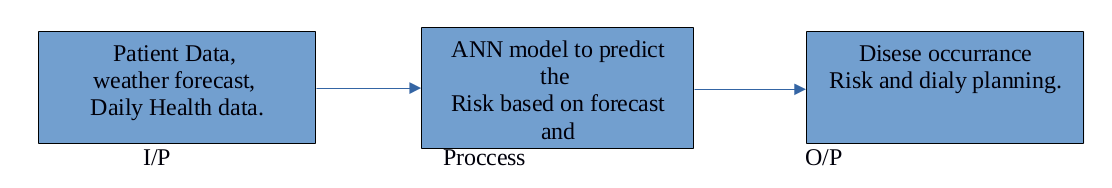
\includegraphics{math.png}}
			\caption{Mathematical model}
	
\end{figure}

\section{NAMES OF CONFERENCES / JOURNALS WHERE PAPERS CAN BE PUBLISHED}
\begin{itemize}
\item IEEE/ACM Conference/Journal 1
\item Conferences/workshops in IITs
\item Central Universities or SPPU Conferences
\item IEEE/ACM Conference/Journal 2
\end{itemize}

\section{PLAN OF PROJECT EXECUTION}

\begin{table}[h]
	
	\caption {Plan of Project Execution}
	\center
	\begin{tabular}{ |p{3cm}|p{3cm}|p{3cm}|p{3cm}|  }
		
		\hline
		From & To & Task & Status\\
		\hline
		27\textendash06\textendash2017 & 30\textendash06\textendash2017 & Group Formation and finalization &  Done\\
		\hline
		
		01\textendash07\textendash2017 & 15\textendash07\textendash2017 & Topic Search & Done\\
		\hline
		
		16\textendash07\textendash2017 & 20\textendash07\textendash2017 & Preliminary Information Gathering &  Done\\
		\hline
		
		21\textendash07\textendash2017 & 28\textendash07\textendash2017 & Project Dicsussion with Project Coordinator and topic finalization &  Done\\
		\hline
		
		01\textendash08\textendash2017 & 25\textendash08\textendash2017 & Synopsis  preparation and submission &  Done\\
		\hline
		
		25\textendash08\textendash2017  & 10\textendash09\textendash2017    & Detailed Literature Survey &  Done\\
		
		
		19\textendash09\textendash2017	&	24\textendash09\textendash2017 & . & .\\
		\hline
		
		10\textendash10\textendash2017 & 30\textendash10\textendash2017 & Preparing Interim report &  Done\\
		\hline
		
		01\textendash11\textendash2017 & 15\textendash12\textendash2017 & Language Study &  In process\\
		\hline
		
		03\textendash01\textendash2018 & 20\textendash01\textendash2018 & Androids Study &  Not Done\\
		\hline
		
		21\textendash01\textendash2018 & 04\textendash03\textendash2018 & Coding and Implementation &  Not Done\\
		\hline
		
		05\textendash03\textendash2018 & 21\textendash04\textendash2018 & Testing &  Not Done\\
		\hline
		
		13\textendash04\textendash2018 & 21\textendash04\textendash2018 & Final Documentation &  Not Done\\
		\hline
		
		25\textendash04\textendash2018 & 20\textendash05\textendash2018 & Final Project Report &  Not Done\\
		\hline		
	\end{tabular}
	
\end{table}



\chapter{\bf{TECHNICAL KEYWORDS}}
\newpage

\section{AREA OF PROJECT}
The area of our project is Machine Learning and Data Mining.
\section{TECHNICAL KEYWORDS}
\textbf{A.Hardware}
\begin{itemize}
	\item risk prediction
	\item Android phone
\end{itemize}
\textbf{B.Architecture}
\begin{itemize}
	\item Client Server Architecture
	\item Realtime Database Connectivity
\end{itemize}
\textbf{C.Networking}
\begin{itemize}
	\item Server 
\end{itemize}


\chapter{INTRODUCTION}
\newpage

\section{PROJECT IDEA}
The overall Idea of the project is to provide user with before hand daily health related risks based on user's daily routine and weather changes as well as historic health data. The project's idea is to formulate a efficient Electronic Health Record so that the prediction is most accurate. 

\section{MOTIVATION OF THE PROJECT}
It is evident from the historic data as well as human knowledge that human general health is closely related to the climatic conditions and the occurrence of diseases is greatly affected by the climate change. This inference gave us the motivation to apply advanced computer science concepts like machine learning and data mining to the health data available to extract certain knowledge and apply it to the current realtime health data so that future occurrence of diseases can be accurately predicted.

\section{LITERATURE SURVEY}
\textbf{1.Data Driven Analytics for Personalized Healthcare Jianying Hu,Adam Perer , and Fei Wang, Springer International Publishing Switzerland 2016 C.A. Weaver et al, Healthcare Information Management Systems- Cases, Strategies, and Solutions, Health Informatics,DOI 10.1007}

The concept of Learning Health Systems (LHS) is gaining momentum as
more and more electronic healthcare data becomes increasingly accessible. The core
idea is to enable learning from the collective experience of a care delivery network
as recorded in the observational data, to iteratively improve care quality as care is
being provided in a real world setting. In line with this vision, much recent research
effort has been devoted to exploring machine learning, data mining and data visualization methodologies that can be used to derive real world evidence from diverse
sources of healthcare data to provide personalized decision support for care delivery
and care management. It gives an overview of a wide range of
analytics and visualization components  have developed, examples of clinical
insights reached from these components, and some new directions are taken.

\textbf{2.Curve relativity analyse for relationship between blood pressure and atmospheric
temperature using Matlab, 2009 International Conference on E-Learning, E-Business, Enterprise Information Systems, and E-Government}
	
Although there are many evidence indicated that human
blood pressure is influenced by atmospheric temperature ,
there are not useful method or tool use to evaluating the
correlation relationship between atmospheric temperature
and BP(blood pressure) still .The paper collected a serial
date of atmospheric temperature and BP which were
recorded by a family .The atmospheric temperature data
were reported by weather bureau and the BP data were
measured by oneself in electronic blood-pressure
meter(HEM6000) .It was made in Japan by OMRON
company . Everyday BP was measured for two times .In the
morning, the blood-pressure was marked for a.m. BP then in
the afternoon ,the blood-pressure was marked for p.m. BP
.there are six groups data we used to experiment. All of them
include a.m. SBP(shrink blood pressure),a.m. DBP(distend
blood pressure), p.m. SBP, p.m. DBP LT(lowest atmospheric
temperature) HT(highest atmospheric temperature) .Each of
them was recorded during 90 days from day to day. The
characters of them are discrete and there are some random
error exist .There are no general methods ready to evaluate
the relationship between them. For evaluating the
relationship between them objectively .The paper used many
methods and analysed from different aspect to make sure
how the correlation degree are among each others 
.

\textbf{3.Various R Programming Tools for Plotting Data, Gregory R. Warnes, Ben Bolker, Lodewijk Bonebakker, Robert
Gentleman, Wolfgang Huber Andy Liaw, Thomas Lumley, Martin
Maechler, Arni Magnusson, Steffen Moeller, Marc Schwartz, Bill
Venables, }

Various R programming tools for plotting data. Calculating and plotting locally smoothed summary function as ('bandplot', 'wapply'), enhanced versions of standard plots ('barplot2', 'boxplot2',
'heatmap.2', 'smartlegend'), manipulating colors ('col2hex', 'colorpanel', 'redgreen',
'greenred', 'bluered', 'redblue', 'rich.colors'),  calculating and plotting two-dimensional data summaries ('ci2d','hist2d'), enhanced regression diagnostic plots ('lmplot2', 'residplot'),
formula-enabled interface to 'stats::lowess' function ('lowess'),
displaying textual data in plots ('textplot', 'sinkplot'),
plotting a matrix where each cell contains a dot whose size
reflects the relative magnitude of the elements ('balloonplot'),
plotting ``Venn'' diagrams ('venn'),
displaying Open-Office style plots ('ooplot'),
plotting multiple data on same region, with separate axes
('overplot'),
plotting means and confidence intervals ('plotCI', 'plotmeans'),
spacing points in an x-y plot so they don't overlap ('space').


\newpage
\textbf{4.A soft-computing ensemble approach (SEA) to forecast Indian summer
monsoon rainfall, Nisha Kurian, a T. Venugopal, b Jatin Singh a and M. M. Ali *
b
a
Skymet Weather Services, Noida, India
Department of Physics, Novosibirsk State University, Russia}

Agriculture is the backbone of the Indian economy and contributes ∼16percent of gross domestic product and about
10percent of total exports. Hence, accurate and timely forecasting of monthly Indian summer monsoon rainfall is very much in
demand for economic planning and agricultural practices. Several methods and models, comprising dynamic and statistical
models and combinations of the two, exist for monsoon forecasting. Here, a multi-model ensemble approach, combined with
an artificial neural networking technique, was used to develop a soft-computing ensemble algorithm (SEA) to forecast the
monthly and seasonal rainfall over the Indian subcontinent. Forecasts using January to May initial conditions along with
observations during 1982–2014 were used to develop the model. The SEA compares well with observations.

\textbf{5.Climate
Change And
Infectious
Diseases}

Changes in infectious disease
transmission patterns are a likely
major consequence of climate
change. It is needed to learn more
about the underlying complex
causal relationships, and apply this
information to the prediction of
future impacts, using more
complete, better validate.

\textbf{6.Extreme Allergies and Global Warming
National wildlife federation, 2010}

Unchecked global warming will worsen respiratory allergies for
approximately 25 million Americans. Ragweed—–the primary allergen
trigger of fall hay fever—–grows faster, produces more pollen per
plant, and has higher allergenic content under increased carbon
dioxide levels. Longer growing seasons under a warmer climate allow
for bigger ragweed plants that produce more pollen later into the fall.
Springtime allergies to tree pollens also could get worse. Warmer
temperatures could allow significant expansion of the habitat
suitable for oaks and hickories, which are two highly allergenic tree
species. Changing climate conditions may even affect the amount of
fungal allergens in the air.
More airborne allergens could mean more asthma attacks for the
approximately 10 million Americans with allergic asthma. Global
warming may also exacerbate air pollution, which interacts with
allergens to trigger more severe asthma attacks. Cities pose the
biggest health threats for asthmatics because the urban heat island
effect can exacerbate both pollen production and air pollution. These
potential impacts of global warming could have a significant
economic impact: allergies and asthma already cost the United
States more than 32 billion annually in direct health care costs and
lost productivity.
Poison ivy also grows faster and is more toxic when carbon dioxide
increases in the atmosphere. More than 350,000 cases of contact
dermatitis from exposure to poison ivy are already reported in the
United States each year. These numbers are likely to increase if
poison ivy grows faster and becomes more abundant. The reactions
may also become more severe because poison ivy produces a more
potent form of urushiol, the allergenic substance, when carbon
dioxide levels are higher.
We must act now to reduce risks for allergy and asthma sufferers.
An essential first step is to reduce global warming pollution to avoid
the worst impacts, and enable allergy sufferers to continue enjoying
the great outdoors. At the same time, states, communities, and
home owners should undertake smart community planning and
landscaping, with attention to allergenic plants and urban heat island
effects, to limit the amount of pollen and other allergens that
become airborne.

\chapter{PROBLEM DEFINITION AND SCOPE}
\newpage
\section{PROBLEM STATEMENT}
In our project we intend to analyse the data available for various patients of certain diseases which are primarily affected by change in daily routine , climate and diet   . from this analysis we recognize certain pattern related to symptoms , cause and treatment of the disease . Based on this analysis we create a model to predict the risks , prevention and precautions to be taken by the patients with similar pattern . Also the prediction will be supported by the climate forecast and current changes in medical health of the patient . Based on the analysed and detected patterns , the current medical health and climate changes to be confronted by the patient we aim to give in advance prediction to the patient . We also intend to provide the precautionary methods . Along with prediction we intend to prompt the patient about taking care of his health based on his personal health status and the climate changes  .

\subsection{Goals and Objectives}
\begin{enumerate}
\item To be able for users to make plans according health preferences.
\item To provide the user with before-hand risk analysis of specific diseases and allergies.
\item To improve general health status of the user.
\end{enumerate}

\subsection{Statement of Scope}
We describe what features are in the scope of the software and what are not in scope of the software to be developed.
\begin{enumerate}
	\item In our project techcare we are attempting to provide risk prediction of occurrence of disease
	and it's progress based on the machine learning model we aim to create . We want to make a system
	which would update the health status of a person daily and tell him to improve or change his
	routines . Also we want to predict and tell the user to take precautions and identify symptoms
	properly . All this is related to the climate change and it's affect on daily health . We're using the
	climate forecast and historical data of the user to do reduction.
	
\end{enumerate}

\chapter{SYSTEM ARCHITECTURE AND REQUIREMENTS}
\newpage
\section{HARDWARE RESOURCES REQUIRED}
\begin{enumerate}
	\item	400MB Hard disk+1GB for Android SDK, emulator system images and caches
	\item	2GB RAM minimum,4GB RAM recommended
	\item	Intel Processor with support for Intel VT-x, Intel EM64T(Intel 64)
	\item	Computer  with windows Vista/7/8/10.
	
\end{enumerate}

\section{SOFTWARE RESOURCES REQUIRED}

\begin{itemize}
	\item Platform: Android SDK
\item  Operating System: Android
\item  Programming Language: python,R.
\item  Tools-R Studio
\item  Packages - keras
\end{itemize}

\newpage
\section{SYSTEM ARCHITECTURE}
\begin{figure}[h]
		\begin{center}
			\scalebox{0.6}{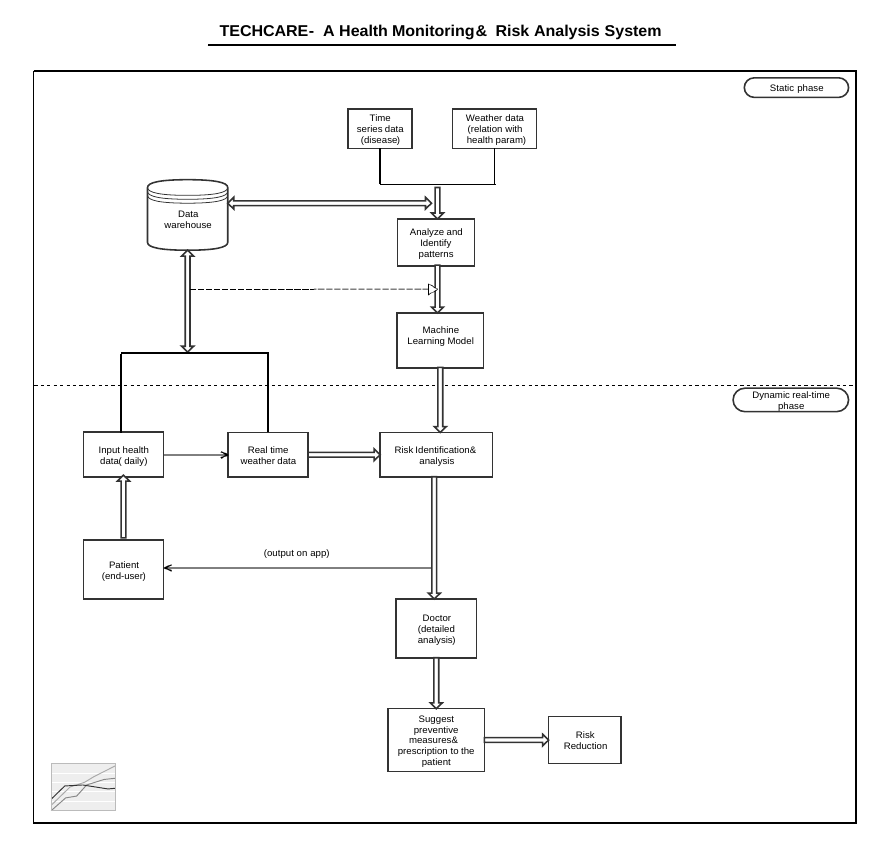
\includegraphics{system.png}}
			\caption{System architecture}
		\end{center}
\end{figure}
\newpage
\chapter{Feasibility study}
\newpage
\section{Technical feasibility}
\subsection{Hardware feasibility}
The hardware components are required mainly to increase the speed of training
the neural network and test time implementation. GPU has also been used to train
the same model and the same dataset which gives an extremely high performance of
training and opens a window for datasets having large number of training examples
or even those datasets having larger number of features.
\subsection{Software feasibility}
The software components used in this project are open source libraries and plat-
forms. Python is the primary programming language used to implement the project.
In order to build neural network models keras open source library has been used
which provides a simpler way to code the model along with open source library for
machine learning which is Tensorflow as a backend for keras implementation. Also
R studio has been used to analyse the data.
\section{Economical feasibility}
The software and the hardware part of the project implementation doesn't require
any cost so far. Due to use of free and open source libraries for deep learning, optimization and preprocessing for the software part which doesn't incur any cost for training the model.
\section{Schedule feasibility}
The solution would be built in an estimated time of 7-8 months.The model
building,training and implementation would be divided into sequential phases as each
component in the project is functionally dependent on the previous one. Time constraints have been imposed for every phase and especially in the phase of increasing
accuracy and fine tuning the parameters of the model and making it more robust.

\section{Operational feasibility}
The system would be used for patients to self test their health and get predictions of diseases based on the changing weather.
\newpage
\chapter{Design}
\newpage
\section{UML modeling}
The Unified Modelling Language (UML) is a general-purpose, developmental, modelling language in the field of software engineering, that is intended to provide a standard
way to visualize the design of a system.UML is a standard language for specifying,
visualizing, constructing, and documenting the artifacts of software systems. UML
was created by Object Management Group and UML 1.0 specification draft was pro-
posed to the OMG in January 1997.
\subsection{Goals of UML:}

\begin{itemize}
\item Provide users with a ready-to-use, expressive visual modeling language so they
can develop and exchange meaningful models.
\item Provide extensibility and specialization mechanisms to extend the core concepts.
\item Be independent of particular programming languages and development pro-
cesses.Integrate best practices
\item Provide a formal basis for understanding the modelling language.
\item Encourage the growth of the OO tools market.
\end{itemize}

\newpage
\subsection{UML diagrams for the project:}
\subsubsection{Use Case diagram}
Use case diagrams are usually referred to as behaviour diagrams used to describe a set of actions (use cases) that some system or systems (subject) should or can perform in collaboration with one or more external users of the system (actors).

	\begin{figure}[h]
		\begin{center}
			\scalebox{0.5}{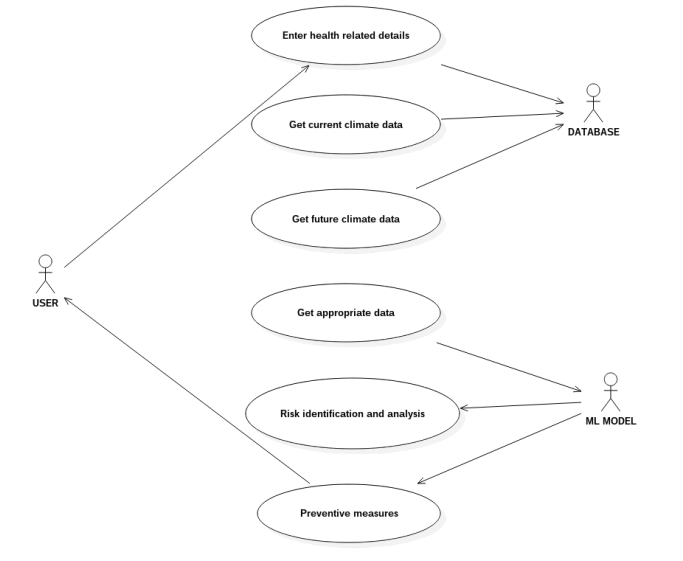
\includegraphics{1.png}}
			\caption{Use Case diagram}
		\end{center}
	\end{figure}

\subsubsection{Activity diagram}
Activity diagrams are graphical representations of workflows of stepwise activities and actions with support for choice, iteration and concurrency. In the Unified Modelling Language, activity diagrams are intended to model both computational and organizational processes (i.e. workflows).\\

\begin{figure}[h]
	\begin{center}
		\scalebox{0.6}{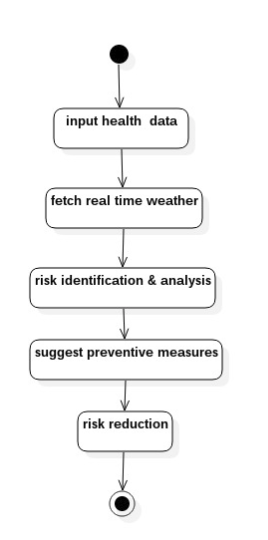
\includegraphics{2.png}}
		\caption{Activity Diagram}
	\end{center}
\end{figure}

\subsubsection{Component diagram}
Component diagram is a special kind of diagram in UML. The purpose is also different from all other diagrams discussed so far. It does not describe the functionality of the system but it describes the components used to make those functionalities.\\

\begin{figure}[h]
	\begin{center}
		\scalebox{0.25}{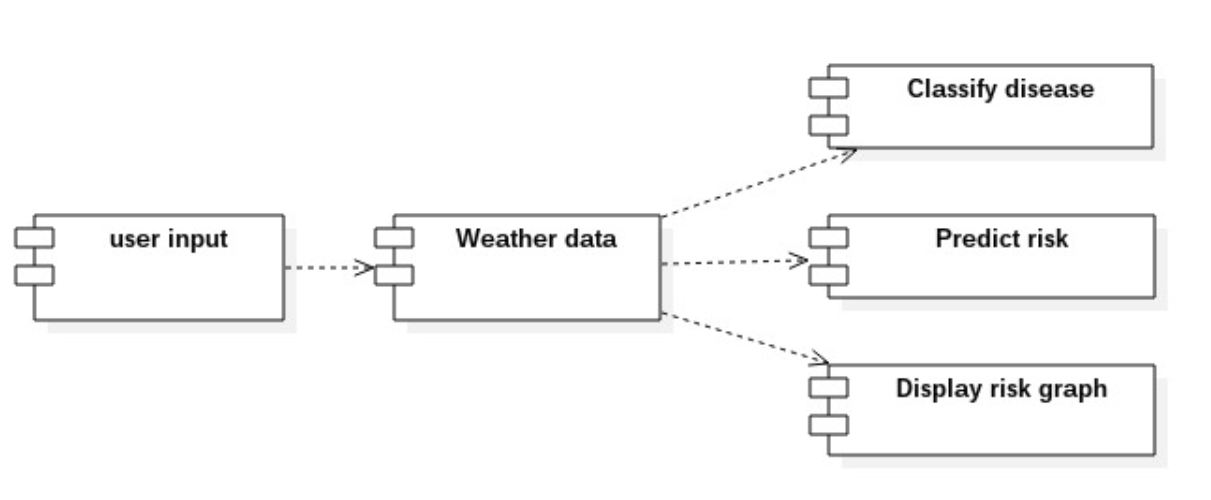
\includegraphics{3.png}}
		\caption{Component Diagram}
	\end{center}
\end{figure}


\subsubsection{Deployment diagram}
Deployment diagram is a structure diagram which shows architecture of the system as deployment (distribution) of software artifacts to deployment targets. Artifacts represent concrete elements in the physical world that are the result of a development process.

\begin{figure}[ht]
	\begin{center}
		\scalebox{0.5}{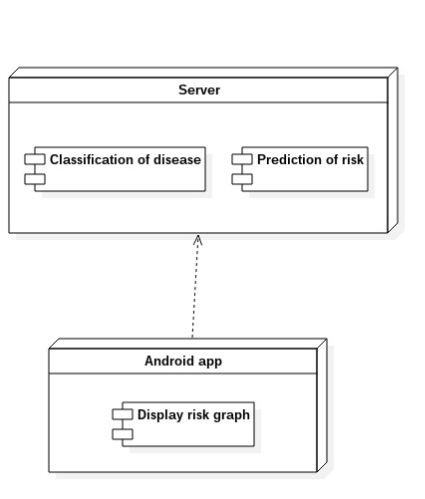
\includegraphics{4.png}}
		\caption{Deployment Diagram}
	\end{center}
\end{figure}
\newpage
\subsubsection{Sequence diagram}
A sequence diagram is an interaction diagram that shows how objects operate with one another and in what order. It is a construct of a message sequence chart. A sequence diagram shows object interactions arranged in time sequence.\\

\begin{figure}[h]
	\begin{center}
		\scalebox{0.5}{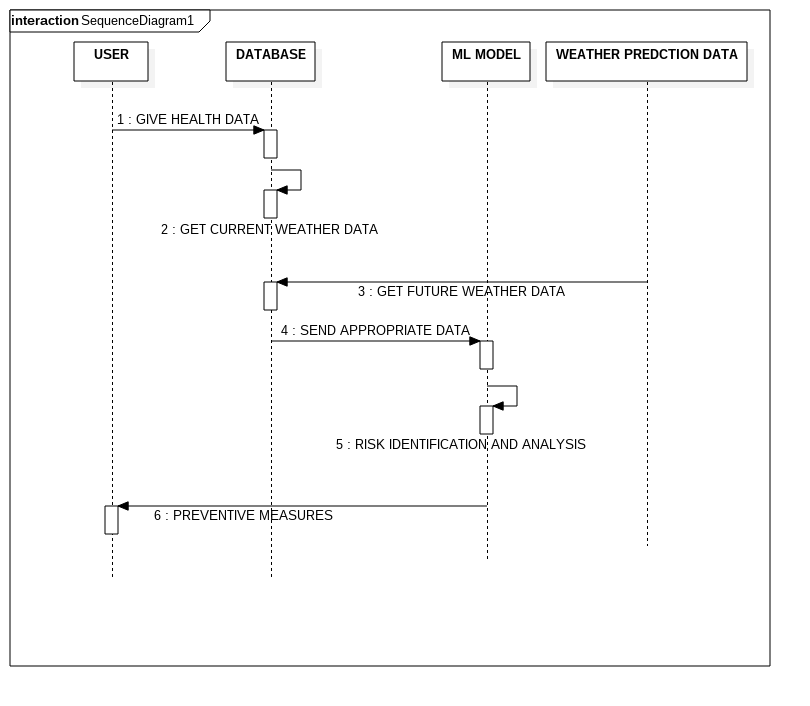
\includegraphics{5.png}}
		\caption{Sequence Diagram}
	\end{center}
\end{figure}
\newpage
\subsubsection{Interaction diagram}
Interaction diagrams are models that describe how a group of objects collaborate in some behavior - typically a single use-case. The diagrams show a number of example objects and the messages that are passed between these objects within the use-case.\\

\begin{figure}[h]
	\begin{center}
		\scalebox{0.5}{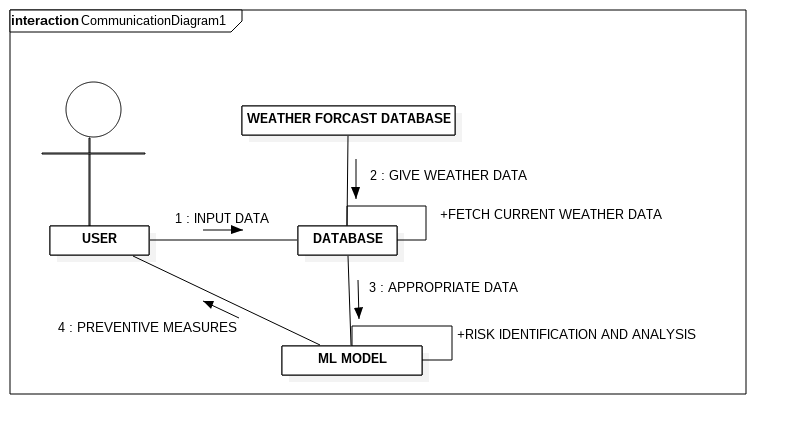
\includegraphics{6.png}}
		\caption{Interaction Diagram}
	\end{center}
\end{figure}


\subsubsection{Statechart diagram}
A state diagram, also called a state machine diagram or statechart diagram, is an illustration of the states an object can attain as well as the transitions between those states in the Unified Modeling Language (UML).\\

\begin{figure}[h]
	\begin{center}
		\scalebox{0.65}{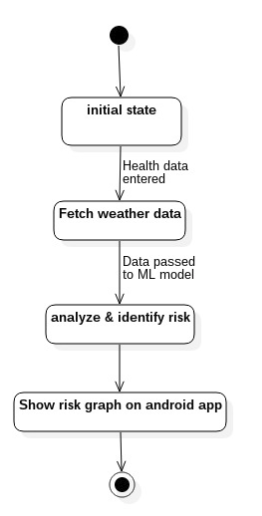
\includegraphics{7.png}}
		\caption{Statechart Diagram}
	\end{center}
\end{figure}

\end{document}
